The TRITIUM-IFIC-1 prototype was designed to correct the problems and limitations found in TRITIUM-IFIC-0. The main improvements were:

\begin{enumerate}

\item{} The fiber bundle was arranged straight to optimize the photon collection efficiency of the fibers. In addition, a PTFE matrix was used to maintain a distance of $1~\mm$ between fibers.

\item{} A special fiber cleaning method, described in section \ref{sec:CharacterizationScintillatingFibers}, was applied to the fibers to improve the quality of the interfaces between fibers and tritiated water. This method produces a better wetting property of the fibers, which improves their photon collection efficiency.

\item{} A PTFE vessel was used to improve the collection of photons inside the prototype. Indeed, PTFE has a reflectivity close to $100\%$ at the fiber scintillating wavelengths. Thus, the photons that escape from fibers and hit the vessel walls are refelcted back into the scintillating fibers.

\end{enumerate}

The TRITIUM-IFIC-1 prototype consists of 64 straight scintillating fibers of $20~\cm$ length, arranged in an $8\times 8$ PTFE squared matrix, as shown in Figure \ref{fig:TeflonStructureFibersTritiumIFIC1}.
\begin{figure}[h]
\centering
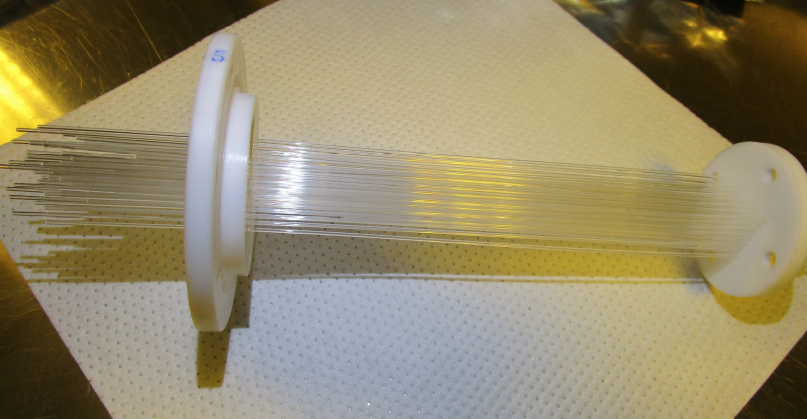
\includegraphics[scale=0.4]{5Prototypes/52PreliminarPrototypes/522TritiumIFIC1/FiberMatrixTeflonStructure.png}
\caption{PTFE structure used to arrange the fibers of TRITIUM-IFIC-1 prototype in a matrix of $8 \times 8$.\label{fig:TeflonStructureFibersTritiumIFIC1}}
\end{figure}
This structure is placed within a cylindrical PTFE vessel of $48~\mm$ diameter and $200~\mm$ length, shown in Figure \ref{fig:TeflonVesselTritumIFIC1}. 
\begin{figure}
\centering
    \begin{subfigure}[b]{0.30\textwidth}
    \centering
    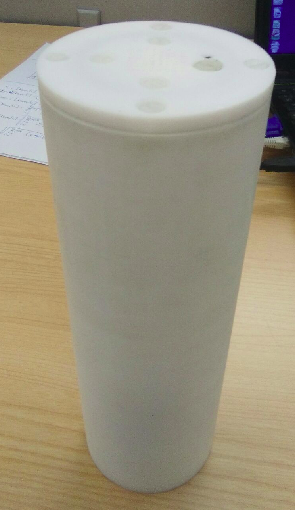
\includegraphics[width=\textwidth]{5Prototypes/52PreliminarPrototypes/522TritiumIFIC1/TeflonVesselTritiumIFIC1a.png}  
    \caption{\label{subfig:TeflonVesselTritumIFIC1a}}
    \end{subfigure}
    \hfill
    \begin{subfigure}[b]{0.45\textwidth}
    \centering
    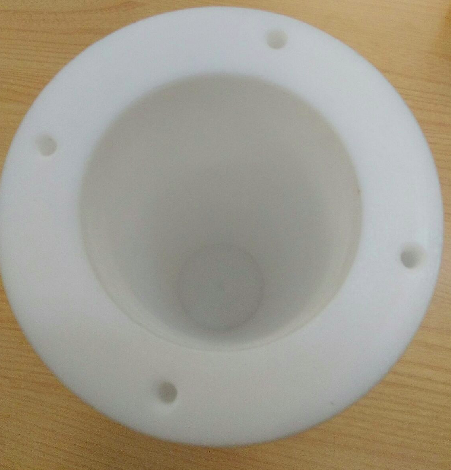
\includegraphics[width=\textwidth]{5Prototypes/52PreliminarPrototypes/522TritiumIFIC1/TeflonVesselTritiumIFIC1b.png}  
    \caption{\label{subfig:TeflonVesselTritumIFIC1b}}
    \end{subfigure}
 \caption{PTFE vessel of TRITIUM-IFIC-1 prototype.}
 \label{fig:TeflonVesselTritumIFIC1}
\end{figure}
The cleaning process described in section \ref{sec:CharacterizationScintillatingFibers} was applied to the fibers to achieve a better tritiated water-fiber interface. A PVC piece was used to attach the photosensor to the prototype and to prevent external light. A general view of this prototype is shown in Figure \ref{fig:TritumIFIC1}.

\begin{figure}[h]
\centering
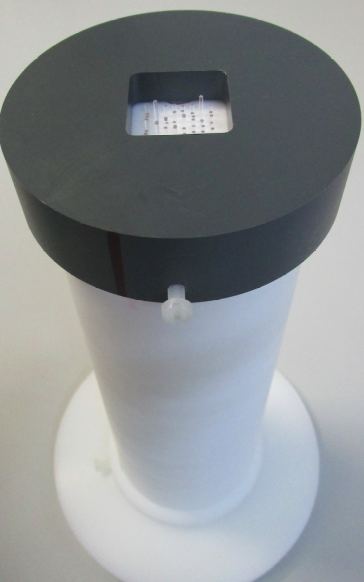
\includegraphics[scale=0.4]{5Prototypes/52PreliminarPrototypes/522TritiumIFIC1/TritiumIFIC1a.png}
\caption{A general view of TRITIUM-IFIC-1 prototype.\label{fig:TritumIFIC1}}
\end{figure}
The prototype was instrumented with a PMT model R8520-460, from Hamamatsu Photonics \cite{DataSheetPMTs}, coupled directly to the fiber bundle by optical grease \cite{OpticalGrease}. The quantum efficiency of this PMT for the fiber scintillating wavelength is $28.66\%$.  The PMT high voltage was $-800~\volt$. The DAQ was the same as for the TRITIUM-IFIC-0 prototype. Only one TRITIUM-IFIC-1 prototype was built. In a first measurement, this prototype was filled with pure water ($118~\milli\liter$, uncertainty of $0.05\%$) and several background measurements were taken during a week. Subsequenty, it was emptied and refilled with $118~\milli\liter$ (uncertainty of $0.05\%$) of tritiated water, $99.696~\kilo\becquerel/\liter$ activity. 

The measured signal and background energy spectra are shown in Figure \ref{subfig:SignalBackgroundEnergySpectraTritiumIFIC1}. The difference between both energy spectra is shown in Figure \ref{subfig:TritiumEnergySpectraTritiumIFIC1}. The rates obtained from the integration of the spectra are given in Table \ref{tab:CountsPerSecondTRITIUMIFIC1}. 

\begin{figure}
\centering
    \begin{subfigure}[b]{1\textwidth}
    \centering
    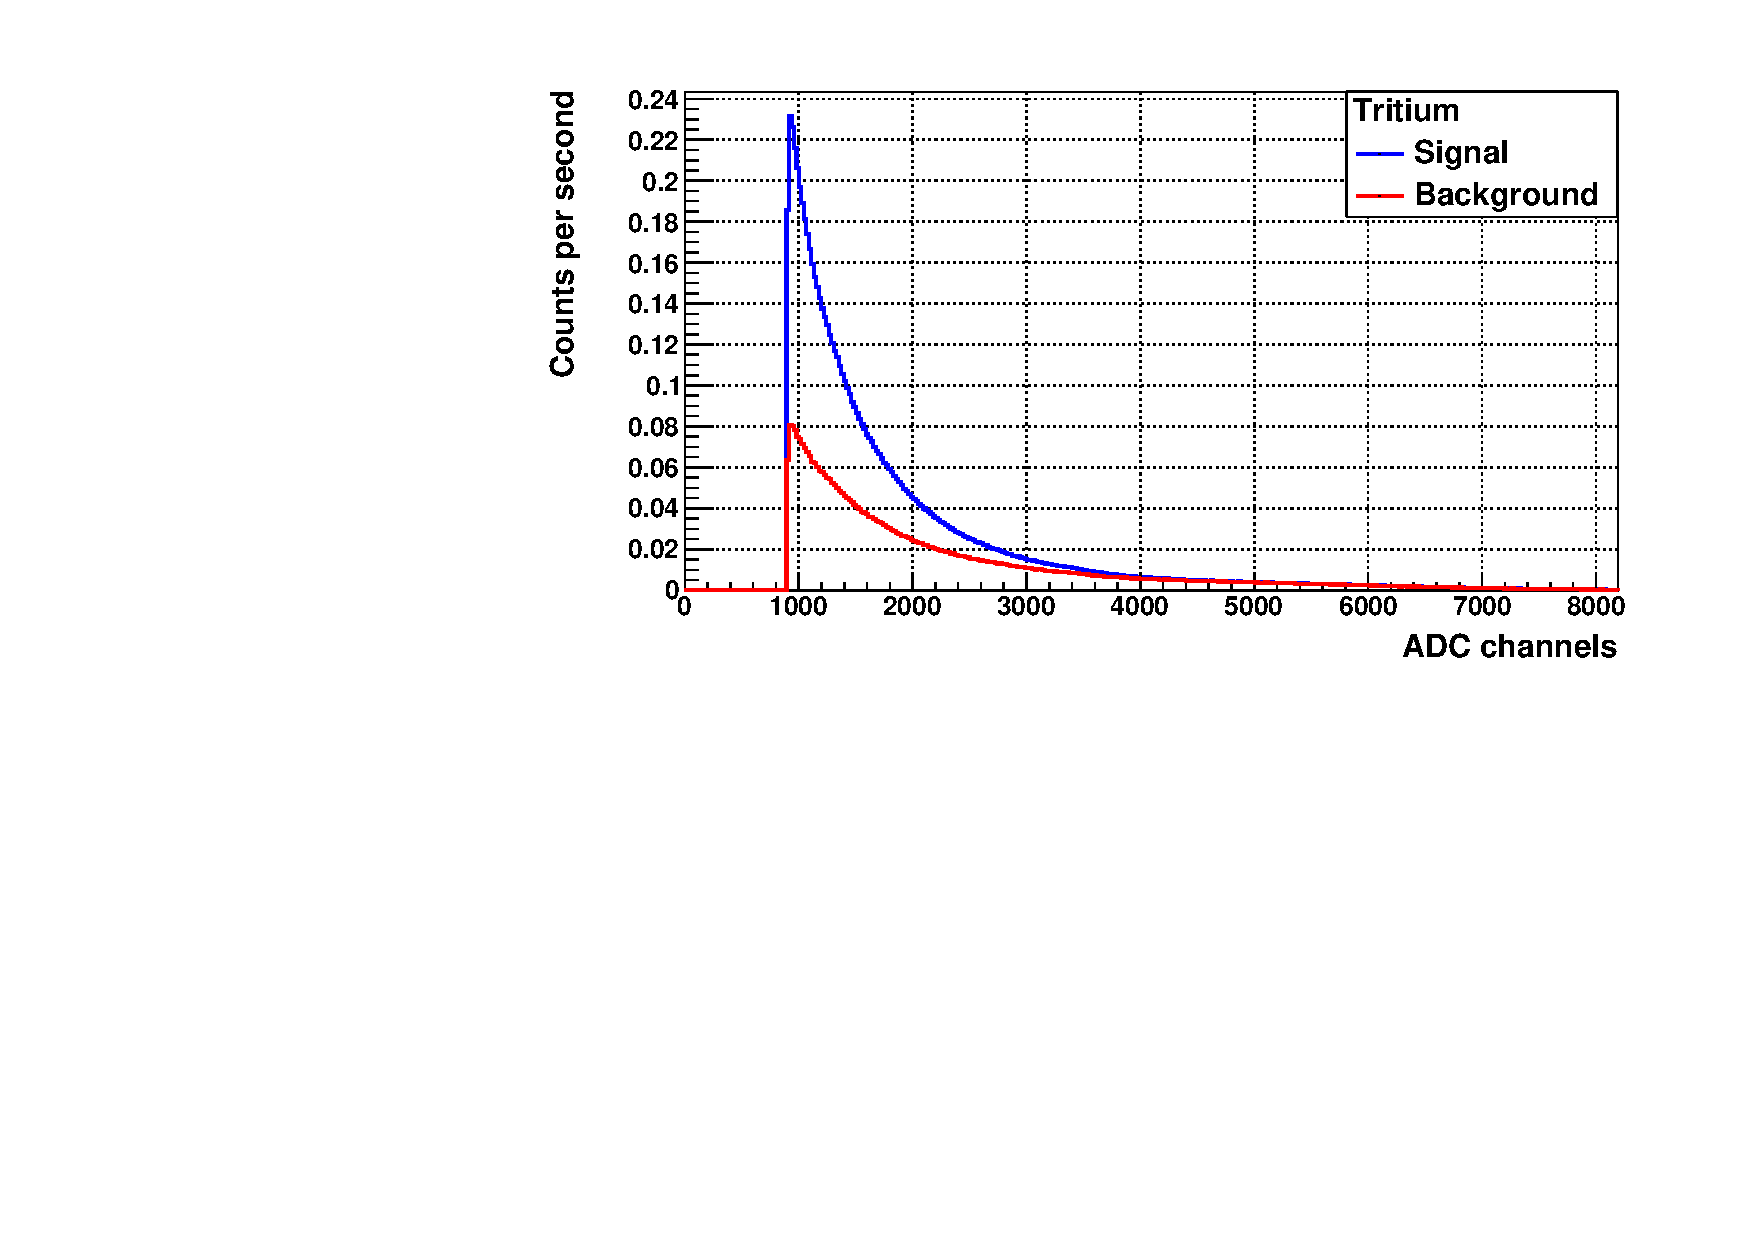
\includegraphics[width=\textwidth]{5Prototypes/52PreliminarPrototypes/522TritiumIFIC1/TritiumIFIC1Signals.pdf}  
    \caption{\label{subfig:SignalBackgroundEnergySpectraTritiumIFIC1}}
    \end{subfigure}
    \hfill
    \begin{subfigure}[b]{1\textwidth}
    \centering
    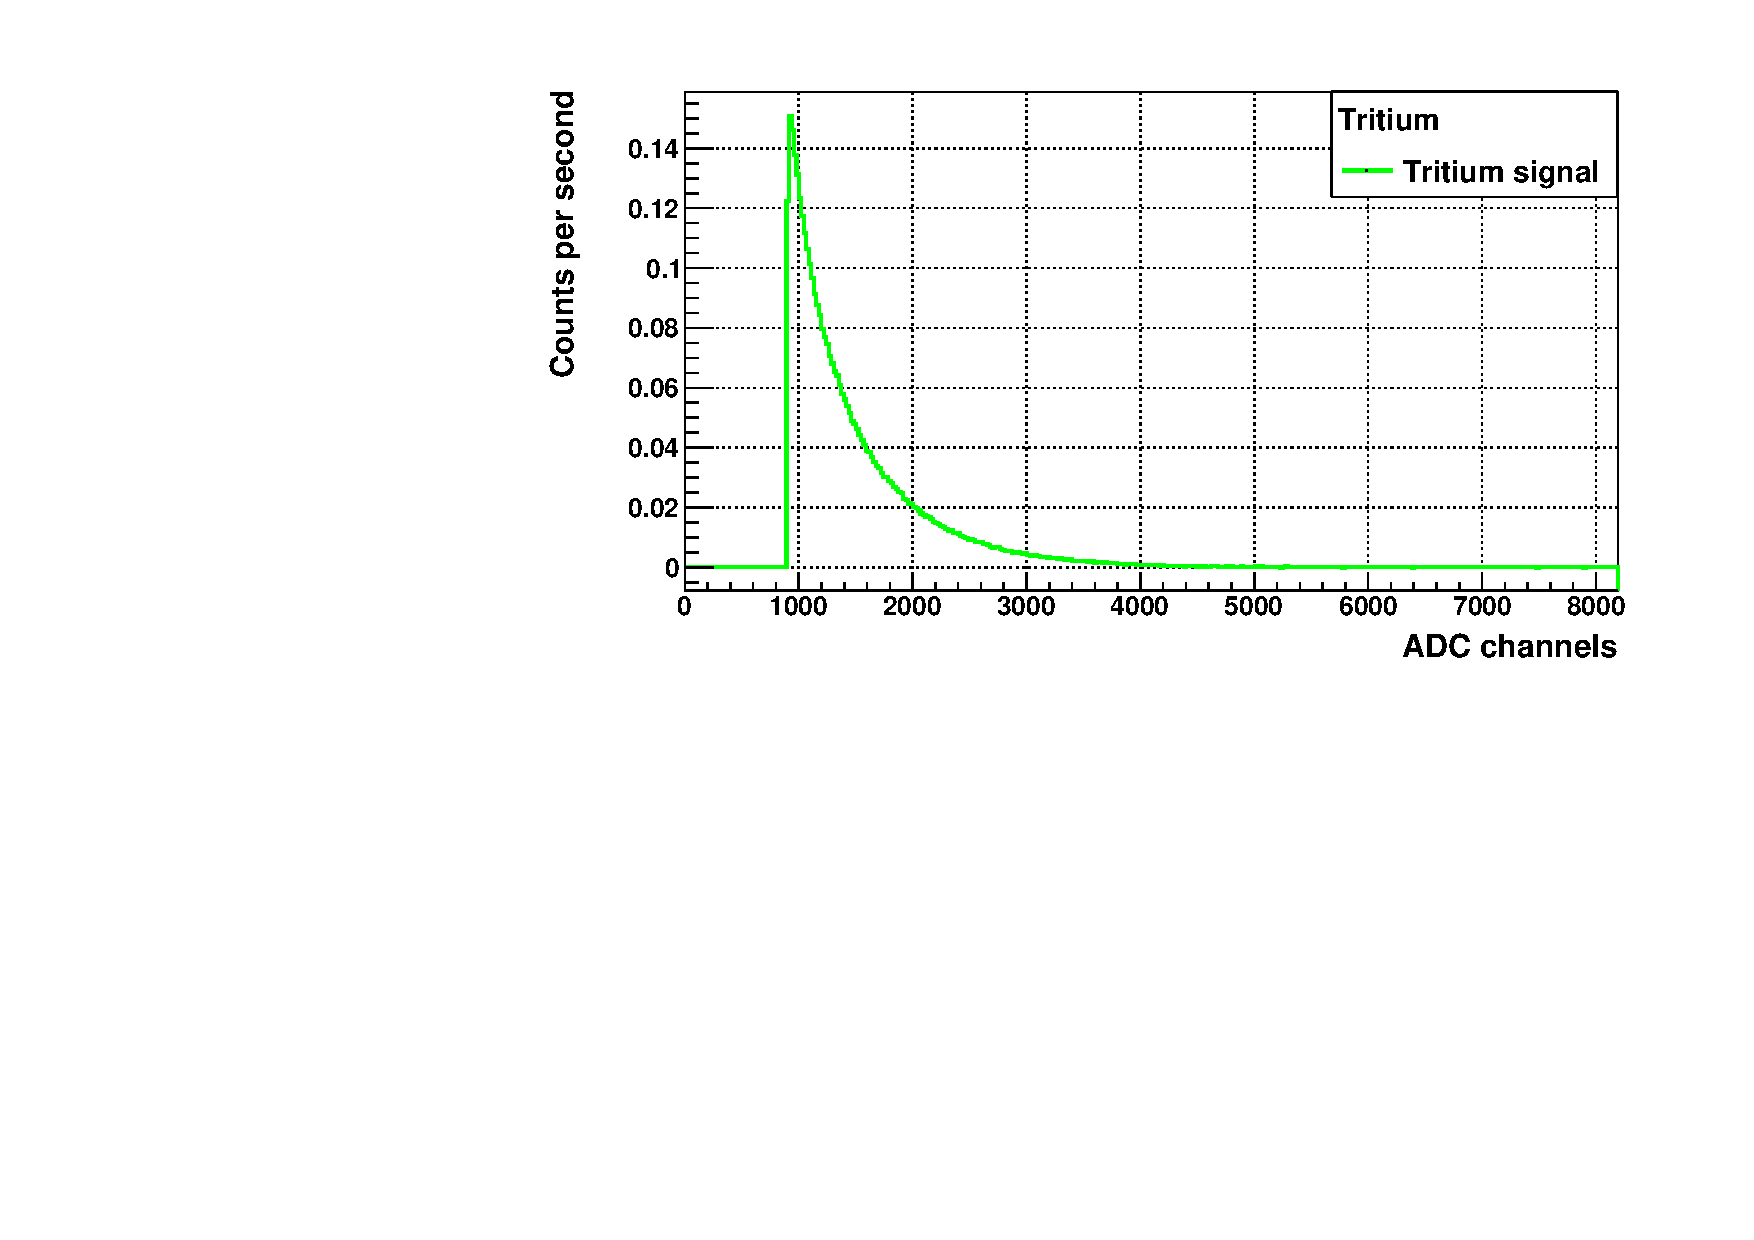
\includegraphics[width=\textwidth]{5Prototypes/52PreliminarPrototypes/522TritiumIFIC1/TritiumIFIC1Clear.pdf}  
    \caption{\label{subfig:TritiumEnergySpectraTritiumIFIC1}}
    \end{subfigure}
 \caption{Energy spectra measured with the TRITIUM-IFIC-1 prototype. a) Signal and background energy spectra. b) Tritium energy spectrum.}
 \label{fig:EnergySpectraTRITIUMIFIC1}
\end{figure}

\begin{table}[htbp]
\centering{}%
\begin{tabular}{cc}
\toprule 
Spectrum & Counts/second \tabularnewline
\midrule
\midrule 
Signal prototype & $7.82 \pm 0.11$ \tabularnewline
Background prototype & $3.99 \pm 0.08$ \tabularnewline  
Tritium counts & $3.83 \pm 0.13$ \tabularnewline
\bottomrule
\end{tabular}
\caption{Counting rate obtained with the TRITIUM-IFIC-1 prototype.}
\label{tab:CountsPerSecondTRITIUMIFIC1}
\end{table}
The tritium detection efficiency obtained for TRITIUM-IFIC-1 is $(3.84 \pm 0.16)\cdot{} 10^{-2}~\liter\:\kilo\becquerel^{-1}\second^{-1}$. The specific efficiency obtained is
$$S=(9.56 \pm 0.40)\cdot{} 10^{-5}~\liter\:\kilo\becquerel^{-1}\second^{-1}\cm^{-2}$$
which is a factor ten better than that of TRITIUM-IFIC-0. Furthermore, compared to the scintillating detectors for tritium in water given in table \ref{tab:PlasticScinTritium}, the efficiency of this prototype is very close to the best result, obtained by Singh \cite{Ratnakaran, Ratnakaran2000}, $4,1 \cdot{} 10^{-2}~\liter\:\kilo\becquerel^{-1}\second^{-1}$, and the specific efficiency, which is the most relevant parameter for comparison, is almost 5 times larger than that obtained by Hofstetter \cite{Hofstetter1, Hofstetter2}, $<22.2 \cdot{} 10^{-6}~\liter\:\kilo\becquerel^{-1}\second^{-1}\cm^{-2}$.
